% Diagrams for RL project (compile with LaTeX)

\usepackage{tikz}
\usetikzlibrary{arrows.meta, positioning}

% RL loop diagram
\newcommand{\RLLoopDiagram}{%
  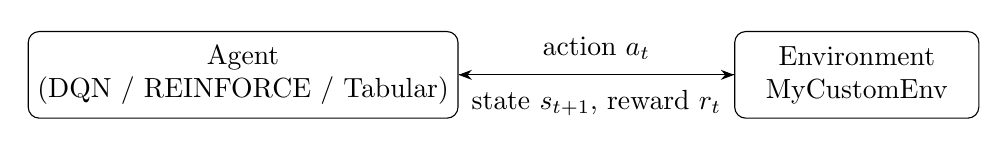
\begin{tikzpicture}[
    node distance=3.5cm,
    >=Stealth,
    box/.style={rectangle, draw, rounded corners, minimum width=3.1cm, minimum height=1.1cm, align=center}
  ]
    \node[box] (agent) {Agent\\(DQN / REINFORCE / Tabular)};
    \node[box, right=of agent] (env) {Environment\\MyCustomEnv};

    % Slightly lifted/lowered labels to avoid overlap with boxes
    \draw[->] (agent) -- node[above,yshift=2pt]{action $a_t$} (env);
    \draw[->] (env)  -- node[below,yshift=-2pt]{state $s_{t+1}$, reward $r_t$} (agent);
  \end{tikzpicture}%
}

% DQN network architecture diagram (high level)
\newcommand{\DQNArchitectureDiagram}{%
  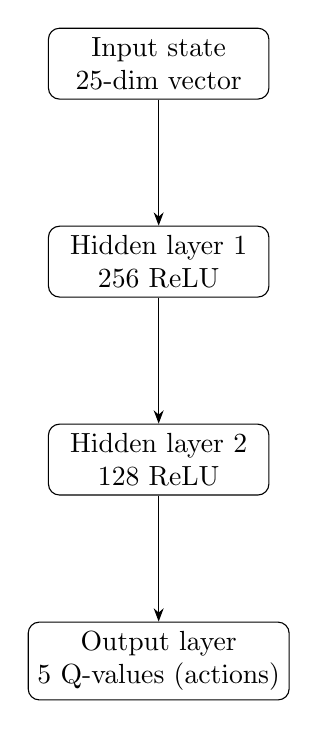
\begin{tikzpicture}[
    node distance=1.6cm,
    >=Stealth,
    layer/.style={rectangle, draw, rounded corners, minimum width=2.8cm, minimum height=0.9cm, align=center}
  ]
    \node[layer] (input) {Input state\\25-dim vector};
    \node[layer, below=of input] (h1) {Hidden layer 1\\256 ReLU};
    \node[layer, below=of h1] (h2) {Hidden layer 2\\128 ReLU};
    \node[layer, below=of h2] (output) {Output layer\\5 Q-values (actions)};

    \draw[->] (input) -- (h1);
    \draw[->] (h1) -- (h2);
    \draw[->] (h2) -- (output);
  \end{tikzpicture}%
}

% Agent comparison conceptual diagram
\newcommand{\AgentComparisonDiagram}{%
  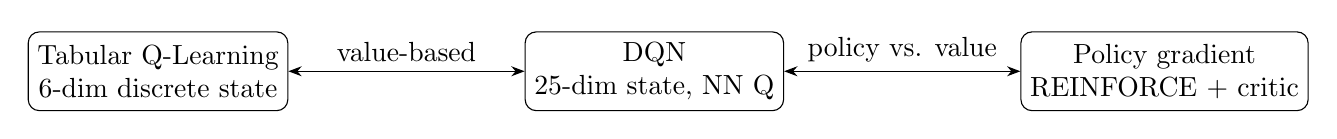
\begin{tikzpicture}[
    node distance=3.0cm,
    >=Stealth,
    box/.style={rectangle, draw, rounded corners, minimum width=2.8cm, minimum height=1cm, align=center}
  ]
    \node[box] (tabular) {Tabular Q-Learning\\6-dim discrete state};
    \node[box, right=of tabular] (dqn) {DQN\\25-dim state, NN Q};
    \node[box, right=of dqn] (reinforce) {Policy gradient\\REINFORCE + critic};

    \draw[<->] (tabular) -- node[above]{value-based} (dqn);
    \draw[<->] (dqn) -- node[above]{policy vs. value} (reinforce);
  \end{tikzpicture}%
}
